\section{Heat kernel expansion}\label{ss:HeatKernel}
The effective action $\log Z_n$ is a one-loop determinant provided that a theory is noninteracting.
The computation of the effective action is carried out in a standard way using the heat kernel method \cite{Birrell:1982ix}.
Here we reexamine a free massive scalar field in $d$ dimensions on $\CM_n$ using this method.
The one-loop effective action is given by
\begin{align}\label{MassiveScalar}
\begin{aligned}
\log Z_n &= - \frac{1}{2} \log \det ( \CD + m^2) \ ,\\
	&= \frac{1}{2} \int_{\epsilon^2}^\infty \frac{\d s}{s}\,  \tr \,K_{\CM_n}(s) \,e^{-m^2 s}\ ,
\end{aligned}
\end{align}
where $\CD$ is a scalar Laplacian plus the scalar curvature $\CD = -\nabla^2 + \xi R$ 
and $m$ is the mass of the scalar field. The parameter $\xi$ is free, but becomes $(d-1)/(4d)$ when the theory is conformally invariant (see Sec. \ref{ss:CFT}).
In the second equality, we used the Schwinger representation and introduced the UV cutoff scale $\epsilon$. 
The {\it heat kernel operator}\footnote{The name follows from the fact that it satisfies the heat equation $(\partial_s + \CD) K_{\CM_n} (s) = 0$.} $K_{\CM_n}(s) = e^{-s \CD}$ has the expansion around $s=0$ of the following form:
\begin{align}\label{HKE}
\tr\, K_{\CM_n} (s) = \frac{1}{(4\pi s)^{d/2}} \sum_{i=0}^\infty a_i(\CM_n)\, s^i \ .
\end{align}
Note that the heat kernel coefficients $a_i$ do not depend on $s$.

As we see shortly, the heat kernel coefficients allow the expansion in the $n \to 1$ limit into the bulk and surface parts on a singular manifold $\CM_n$,
\begin{align}\label{HKCoefficient}
a_i = a_i^\text{bulk} + (1-n) \,a_i^\Sigma + O\left( (1-n)^2\right)\ .
\end{align}
The bulk part $a_i^\text{bulk}$ for the $n$-fold cover $\CM_n$ is $n$ times larger than the one for the original space $\CM_1$
\begin{align}\label{BulkMn}
a_i^\text{bulk}(\CM_n) = n\, a_i^\text{bulk}(\CM_1) \ .
\end{align}
The subleading terms arise from the contributions of the conical singularity at the hypersurface $\Sigma$.
Using the heat kernel expansion Eq.\,\eqref{HKE} in the effective action Eq.\,\eqref{MassiveScalar}, we obtain the entanglement entropy as a power series of the inverse of the mass with the heat kernel coefficients,
\begin{align}\label{EE_Scalar_HK}
S_A = \frac{1}{2(4\pi)^{d/2}}\sum_{i=0}^\infty \frac{a_i^\Sigma}{m^{2i - d}} \,\Gamma\left( i - \frac{d}{2}, m^2 \epsilon^2\right) \ ,
\end{align}
where $\Gamma(a,z)$ is the incomplete gamma function defined by $\Gamma (t,x) = \int_x^\infty \d s\, s^{t-1} e^{-s}$.
Hence given the surface parts of the heat kernel coefficients, the entanglement entropy is calculable at any order of the heat kernel expansion.\footnote{The heat kernel method may be adapted to the perturbative studies of R{\'e}nyi entropy near $n=1$, which requires the subleading coefficients in the expansion Eq.\,\eqref{HKCoefficient}.}

We fix the heat kernel coefficients following the strategy used by \textcite{Fursaev:1994in,Fursaev:1995ef,Fursaev:2013fta} [see also \textcite{Solodukhin:2011gn} for a review].
First, we start with the known results for the bulk heat kernel coefficients on a nonsingular manifold $\CM$ \cite{Birrell:1982ix,Vassilevich:2003xt}:
\begin{align}\label{HKbulk}
\begin{aligned}
a_0^\text{bulk} &= \int_{\CM} 1\ , \\
	a_1^\text{bulk} &= \left( \frac{1}{6} - \xi \right) \int_{\CM} \CR \ , \\
	a_2^\text{bulk} &= \int_{\CM} \left[ \frac{1}{180} \CR_{\mu\nu\rho\sigma}^2 - \frac{1}{180} \CR_{\mu\nu}^2 \right.\\
		&\qquad \qquad \left. + \frac{1}{2}
	 \left( \frac{1}{6} - \xi \right)^2 \CR^2 + \frac{1}{6} \left( \frac{1}{5} - \xi \right)\nabla^2 \CR \right]\ .
\end{aligned}
\end{align}
To obtain the surface parts, we regularize the conical singularity at $\Sigma$ and replace $\CM_n$ with a regularized manifold $\widetilde \CM_n$.
Eqs.\,\eqref{HKbulk} are valid for the smooth geometry $\widetilde \CM_n$ from which we read off the surface parts $a_i^\Sigma$.



\subsection{Regularized cone with $\U(1)$ symmetry}\label{ss:RegConeU(1)}
Before presenting general cases, we consider a two-dimensional cone $\CC_n$ with a conical singularity at the origin (we denote it by $\Sigma$),
\begin{align}
\begin{aligned}
\d s^2_{\CC_n} &= e^{\sigma (r)} (\d r^2 + r^2 \d\tau^2) \ , \\
\sigma(r) &= \sigma_1 r^2 + \sigma_2 r^4 + \cdots \ ,
\end{aligned}
\end{align}
where $0\le r \ ,  0\le \tau \le 2\pi n$, and $\sigma_1$ and $\sigma_2$ are constant.
It has a deficit angle $2\pi(1-n)$ at the tip. 


In order to properly take into account the singularity, we regularize the cone by deforming the metric so that the origin at $r=0$ becomes smooth while it has the same geometry as $\CC_n$ away from $\Sigma$.
We call such a geometry \emph{a regularized cone} $\tilde \CC_n$, letting the metric be 
\begin{align}\label{RegCone}
\d s^2_{\tilde \CC_n} = e^{\sigma (r)} \left[ f_\delta (r)\, \d r^2 + r^2 \d \tau^2 \right] \ ,
\end{align}
where $f_\delta (r)$ is a smooth function satisfying
\begin{align}\label{SmoothingFunction}
f_\delta (r \to 0) = n^2 \ , \qquad f_\delta (r>\delta) = 1 \ ,
\end{align}
with a small parameter $\delta \ll 1$.\footnote{The small parameter $\delta$ has nothing to do with the UV cutoff $\epsilon$ in general and can be tuned arbitrarily.}
The regularized cone $\tilde\CC_n$ agrees with $\CC_n$ for $r> \delta$ and becomes flat space at $r=0$ as illustrated in Fig.\,\ref{fig:RegCone}.

\begin{figure}[htbp]
\centering
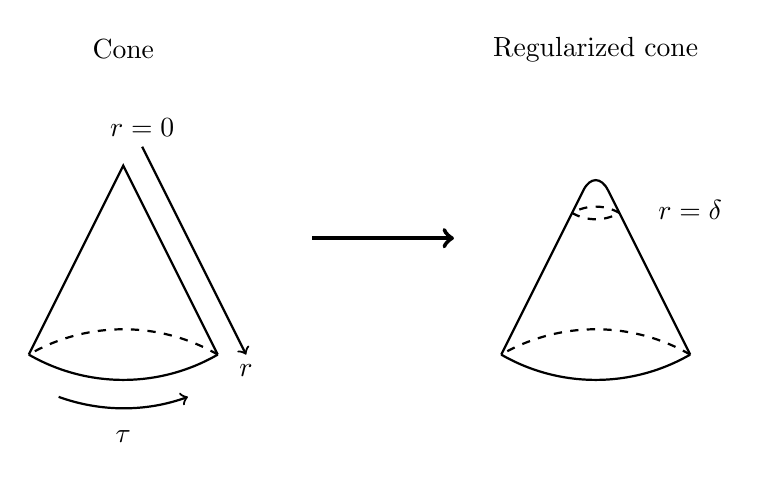
\begin{tikzpicture}[scale=1.2]
	\draw [thick] ([shift=(240:2)]1,2) --++ (1,2) -++ (1,-2);
	\draw [thick] ([shift=(240:2)]1,2) arc (240:300:2);
	\draw [thick, dashed] ([shift=(300:2)]1,2) arc (60:120:2);
	\draw [thick, ->] ([shift=(240:2)]2.2,4.2) node [above] {$r=0$} --++ (1.1,-2.2) node [below] {$r$};
	\draw [thick, ->] ([shift=(250:2)]1,1.7) arc (250:290:2);
	\node at (1,-0.6) {$\tau$};
	\node at (1,3.5) {Cone};
	
	\draw[ultra thick, ->] (3,1.5) --++ (1.5,0);
	
	\draw [thick, rounded corners=10] ([shift=(240:2)]6,2) --++ (1,2) -++ (1,-2);
		
	\draw [thick, dashed] ([shift=(240:0.5)]6,2.2) arc (240:300:0.5);
	\draw [thick, dashed] ([shift=(300:0.5)]6,2.2) arc (60:120:0.5);
	\draw [thick] ([shift=(240:2)]6,2) arc (240:300:2);
	\draw [thick, dashed] ([shift=(300:2)]6,2) arc (60:120:2);
	\node at (7,1.8) {$r=\delta$};
	\node at (6,3.5) {Regularized cone};
\end{tikzpicture}
\caption{A cone that has a singularity at $r=0$ is smoothened by replacing the tip with a disk.}
\label{fig:RegCone}
\end{figure}


Next we evaluate the Riemann tensors $\CR_{\mu\nu\rho\sigma}$ on $\tilde \CC_n$.
Since the Riemann tensor in two dimensions is fixed by the Ricci scalar,
\begin{align}
	\CR_{\mu\nu\rho\sigma} = \frac{\CR}{2}(g_{\mu\rho} g_{\nu\sigma} - g_{\mu\sigma} g_{\nu\rho}) \ ,
\end{align}
it is enough to calculate $\CR$ on $\tilde \CC_n$.
The Ricci scalar for the metric \eqref{RegCone} is given by
\begin{align}
	\CR = e^{-\sigma} \left( \frac{f_\delta'}{r f_\delta^2} - \frac{\partial_r^2 \sigma}{f_\delta} \right) \ .
\end{align}
The first term in the bracket of the right-hand side, representing a contribution to the Ricci curvature from the singularity, naively vanishes when $\delta = 0$.
However, it contributes to the integral as a surface term even in $\delta \to 0$ limit as seen from the integral of the Ricci scalar,
\begin{align}
\begin{aligned}
\int_{\tilde\CC_n} \CR &= 2\pi n\int_0^\infty \d r \left[ -2 \partial_r f^{-1/2}_\delta(r) - r f_\delta^{-1/2}(r) \, \partial_r^2 \sigma \right] \ ,\\
	&= 4\pi (1-n) - 2\pi n \int_0^\infty \d r \,r f_\delta^{-1/2}(r) \, \partial_r^2 \sigma \ .
\end{aligned}
\end{align}
The first term proportional to $n-1$ is the contribution of the singularity to the curvature
while the second term is the bulk contribution accounting for the curvature of $\CC_n$ away from the singularity.
Taking the $\delta \to 0$ limit, the second term approaches the integral of the Ricci scalar on the cone $\CC_n$ with the origin $\Sigma$ removed:
\begin{align}
	\lim_{\delta \to 0} \int_{\tilde\CC_n}  \CR = \int_{\CC_n/\Sigma} \CR + 4\pi (1-n)\ .
\end{align}
The final result does not depend on the choice of the smooth function $f_\delta(r)$, thus is independent of the regularization scheme.

This argument can be equally generalized to higher-dimensional theories if the $n$-fold cover $\CM_n$ has a $\U(1)$ symmetry around $\Sigma$, namely if the metric is of the form,
\begin{align}\label{U(1)metric}
	\d s^2_{\CM_n} = e^{\sigma (r)} \left[ \d r^2 + r^2 \d\tau^2 + \gamma_{ij}(r, y)\, \d y^i \d y^j \right] \ ,
\end{align}
where $y^i~(i=1,\cdots, d-2)$ are the coordinates of the entangling surface $\Sigma$ located at $r=0$.
This is actually the case when $\Sigma$ does not have an extrinsic curvature as we see in the next section.
The regularized space $\widetilde \CM_n$ is obtained by replacing the cone with $\tilde \CC_n$, being the product manifold $\tilde \CC_n \times \Sigma$ near $\Sigma$.
We do not reproduce the derivation, but
the results are conveniently summarized in the following relations \cite{Fursaev:1995ef}:
\begin{align}\label{Formula}
\begin{aligned}
	\CR\big|_{\widetilde\CM_n} &= \CR\big|_{\CM_1} + 4\pi (1-n)\, \delta_\Sigma \ , \\
	\CR_{\mu\nu}\big|_{\widetilde\CM_n} &= \CR_{\mu\nu}\big|_{\CM_1} + 2\pi (1-n) N_{\mu\nu}\, \delta_\Sigma \ ,\\
	\CR_{\mu\nu\rho\sigma}\big|_{\widetilde\CM_n} &= \CR_{\mu\nu\rho\sigma}\big|_{\CM_1} \\
		&\qquad + 2\pi (1-n) (N_{\mu\rho}N_{\nu\sigma}-
	N_{\mu\sigma}N_{\nu\rho})\, \delta_\Sigma \ ,
\end{aligned}
\end{align}
where $\delta_\Sigma$ is the delta function for the entangling surface $\Sigma$ and $N_{\mu\nu}$ is defined by  $N_{\mu\nu}= \sum_{a=1}^2 n^a_\mu n^a_\nu$ with the normal vectors $n^a_\mu~(a=1,2)$ to the surface.

As an example, let us apply Eq.\,\eqref{Formula} to the Euler density  defined in $2m$ dimensions by
\begin{align}\label{EulerDensity}
\begin{aligned}
	E_{2m} = \frac{1}{2^{2(m+1)}\pi^m\, m!}\, &\epsilon_{\mu_1\mu_2\cdots \mu_{2m-1}\mu_{2m}} \epsilon^{\nu_1\nu_2\cdots \nu_{2m-1}\nu_{2m}}\\
		&\cdot \CR^{\mu_1\mu_2}_{~~~~~~\nu_1\nu_2} \cdots \CR^{\mu_{2m-1}\mu_{2m}}_{~~~~~~~~~~\nu_{2m-1}\nu_{2m}}  \ .
\end{aligned}
\end{align}
The integral of the Euler density over a manifold $\CM$ is called the Euler invariant $\chi[\CM] \equiv \int_{\CM} E_{2m}$ that is a topological invariant.
It is normalized so that $\chi[\BS^{2m}] = 2$ for an even-dimensional sphere.
Then the application of Eq.\,\eqref{Formula} to Eq.\,\eqref{EulerDensity} yields an interesting relation between the Euler densities of the $n$-fold cover $\widetilde \CM_n$ and the entangling surface $\Sigma$ \cite{Fursaev:1995ef}:
\begin{align}\label{EulerFormula}
	E_{2m}\big|_{\widetilde\CM_n} &= E_{2m}\big|_{\CM_1} + (1-n)\, E_{2m-2}\big|_{\Sigma} + O\left((1-n)^2\right)\ .
\end{align}
Although these relations are likely to hold for the case even without $\U(1)$ symmetry, to our best knowledge, there is no general proof so far.




\subsection{Regularized cone without $\U(1)$ symmetry}\label{ss:Reg_Cone_no_U(1)}
Without a $\U(1)$ symmetry around the entangling surface, the metric can take a more general form than Eq.\,\eqref{U(1)metric}.
If we parametrize the two-dimensional transverse directions to $\Sigma$ by $x_a$ $(a=1,2)$, the manifold $\CM$ looks like a product form $\BR^2 \times \Sigma$ near the origin $x_1=x_2 = 0$.
Even away from the origin, we can still control the metric in the so-called Riemann normal coordinates \cite{Lewkowycz:2013nqa,Fursaev:2013fta,Rosenhaus:2014woa},
\begin{align}
\begin{aligned}
	\d s^2_{\CM} &=  \delta_{ab}\, \d x^a \d x^b + \left(\gamma_{ij}(y) + 2\CK^a_{ij} \, x^a \right) \d y^i \d y^j + O(x^2) \ .
\end{aligned}
\end{align}
We introduced the extrinsic curvature $\CK^a_{\mu\nu}$ by
\begin{align}\label{ExtrinsicCurvature}
\CK^a_{\mu\nu} = h_\mu^{~\rho} h_\nu^{~\sigma} \nabla_\rho n^a_\sigma \big|_{\Sigma}\ , 
\end{align}
where $h$ is the induced metric on $\Sigma$, $h_{\mu\nu} = g_{\mu\nu} - \sum_{a=1}^2 n^a_\mu n^a_\nu$ with the unit normal vector $n^a_\mu = \delta^a_\mu$ to $\Sigma$.
Moving to the polar coordinates $x_1 = r\sin\tau, x_2 = r\cos\tau$, the metric becomes 
\begin{align}
\begin{aligned}
	\d s^2_{\CM} &= \d r^2 + r^2 \d\tau^2 \\
		&\qquad + \left( \gamma_{ij}(y) + 2r \cos\tau\, \CK^1_{ij} + 2r \sin\tau\,\CK^2_{ij} \right) \d y^i \d y^j\\
		&\qquad\quad + O(r^2)\ .
\end{aligned}
\end{align}
The $\U(1)$ symmetry is broken due to the explicit dependence on the angular coordinate $\tau$.
Compared with Eq.\,\eqref{U(1)metric} for $n=1$, the extrinsic curvature $\CK^a_{ij}$ has to vanish when the $\U(1)$ symmetry is present.

We want to calculate the integrals of geometric invariants on the $n$-fold cover as in the $\U(1)$ symmetric case.
To this end, we use the regularized $n$-fold cover $\widetilde\CM_n$ proposed by \textcite{Fursaev:2013fta},
\begin{align}
\begin{aligned}
	&\d s^2_{\widetilde\CM_n^\text{(FPS)}} \\
	&\quad = f_\delta (r) \d r^2 + r^2 \d \tau^2 \\
		&\qquad + \left[ \gamma_{ij}(y) + 2r^n c^{1-n}\left( \cos\tau\, \CK^1_{ij} + \sin\tau\,\CK^2_{ij}\right) \right] \d y^i \d y^j \\
		&\qquad \quad  + O(r^2)\ ,
\end{aligned}
\end{align}
where $\tau\sim\tau + 2\pi n$, $c$ is a constant of dimension of length, and $f_\delta(r)$ is the smoothing function Eq.\,\eqref{SmoothingFunction}.
Using the regularized metric, the following formulas for the integrals of the Riemann curvatures are argued to hold based on several explicit calculations \cite{Fursaev:2013fta}:
\begin{align}
\int_{\widetilde\CM_n} \CR &= n \int_{\CM} \CR + 4\pi (1-n) \int_\Sigma 1 \ ,\label{SingularFormulae1}\\
\int_{\widetilde\CM_n} \CR^2 &= n \int_{\CM} \CR^2 + 8\pi (1-n) \int_\Sigma 
\CR \ , \label{SingularFormulae2}\\
\int_{\widetilde\CM_n} \CR_{\mu\nu}^2 &= n \int_{\CM} \CR_{\mu\nu}^2 \nonumber\\
	&\qquad + 4\pi (1-n) \int_\Sigma \left[\CR_{aa} - \frac{1}{2}(\CK^{a\,\mu}_{\,\mu})^2\right] \ , \label{SingularFormulae3}\\
\int_{\widetilde\CM_n} \CR_{\mu\nu\rho\sigma}^2 &= n \int_{\CM} \CR_{\mu\nu\rho\sigma}^2 \nonumber\\
	&\qquad + 8\pi (1-n) \int_\Sigma \left[ \CR_{abab} - \CK^a_{\mu\nu} \CK^{a\, \mu\nu} \right] \ , \label{SingularFormulae4}
\end{align}
where Eq.\,\eqref{SingularFormulae1} is exact while only the terms up to $O(1-n)$ are shown in the rest.
The subleading integral are performed on the codimension-two surface $\Sigma$ and $\CR_\Sigma$, $\CR_{aa}$ and $\CR_{abab}$ are the Ricci scalar for the induced metric $h$, the induced Ricci tensor $\CR_{aa} = \sum_{a=1,2} n^a_\mu n^a_\nu \CR^{\mu\nu}$ and the induced Riemann tensor $\CR_{abab} = \sum_{a,b=1,2} n^a_\mu n^b_\mu n^a_\rho n^b_\sigma \CR^{\mu\nu\rho\sigma}$, respectively.
These are enough to fix the heat kernel coefficients $a_i$ in Eq.\,\eqref{HKbulk} up to second order.

The results given in Eq.\,\eqref{SingularFormulae1}-\eqref{SingularFormulae4} can be used to derive a similar relation to Eq.\,\eqref{EulerFormula}, but in the integrated forms in two and four dimensions:
\begin{align}\label{EulerFormula2}
	\chi [\widetilde \CM_n] = \chi [\CM] + (1-n) \chi[\Sigma] + O\left((1-n)^2\right)\ ,
\end{align}
where we used the fact that the regularized $n$-fold cover $\widetilde \CM_n$ is topologically the same as the original manifold $\CM$.


\subsection{Heat kernel coefficients}
We move onto the determination of the heat kernel coefficients for the surface parts.
Substituting Eqs.\,\eqref{SingularFormulae1}-\eqref{SingularFormulae4} into the coefficients \eqref{HKbulk} on the smooth geometry $\widetilde\CM_n$,
one finds the bulk parts satisfy Eq.\,\eqref{BulkMn} and the surface parts become \cite{Fursaev:2013fta}
\begin{align}\label{HKsurf}
\begin{aligned}
a_0^\Sigma &= 0\ , \\
	a_1^\Sigma &=  \frac{2\pi (1-6\xi) }{3} \int_\Sigma 1 \ , \\
	a_2^\Sigma &= \frac{\pi}{9} \int_\Sigma \Bigg[ \frac{1}{5} \left( 2 \CR_{abab} - \CR_{aa}  -2 \CK^a_{\mu\nu} \CK^{a\, \mu\nu} + \frac{1}{2}(\CK^{a\,\mu}_{\,\mu})^2\right) \\
		&\qquad \qquad\qquad + (1-6\xi)^2 \CR \Bigg]\ ,
\end{aligned}
\end{align}
where we used the Gauss-Codazzi equation to simplify the expression,
\begin{align}\label{GaussCodazzi}
\CR =  \CR_\Sigma + 2\CR_{aa} - \CR_{abab} - (\CK^{a\,\mu}_{\,\mu})^2 + \CK^a_{\mu\nu} \CK^{a\, \mu\nu} \ .
\end{align}

It follows that the entanglement entropy Eq.\,\eqref{EE_Scalar_HK} for a free massive scalar field has the UV divergences:
\begin{align}\label{EAfinite}
S_A &= \frac{(1-6\xi)}{6(d-2) (4\pi)^{d/2 -1}} \,\frac{A_\Sigma}{\epsilon^{d-2}} + \frac{c_{d-4}}{\epsilon^{d-4}}  + \cdots +\gamma(m) \ ,
\end{align}
where $\gamma(m)$ includes all the mass dependences.
The area law divergence can be found in the leading term that comes from the coefficient $a_1^\Sigma$ proportional to the area $A_\Sigma$ of the surface $\Sigma$. 
In addition, there is a universal term proportional to the area in $\gamma(m)$ \cite{Hertzberg:2010uv}:
\begin{align}\label{gamma_odd}
	\gamma(m) = (1-6\xi)\,\gamma_d \, A_\Sigma\, m^{d-2} + \cdots \ ,\quad \gamma_d = 	\frac{\Gamma(1-d/2)}{12(4\pi)^{d/2-1}} \ .
\end{align}
The coefficient $\gamma_d$ is finite for odd $d$, but is divergent due to the pole of the gamma function for even $d$.
This divergence signals the conformal anomaly in even dimensions and modifies the mass expansion of $\gamma(m)$  for even $d_e$,
\begin{align}
\begin{aligned}
	\gamma(m) =\,& (1-6\xi)\,\gamma_{d_e}^{(\text{even})}\, A_\Sigma\, m^{d_e-2}\log (m\,\epsilon) + \cdots \ , \\
	&\gamma_{d_e}^{(\text{even})} = \frac{(-1)^{d_e/2 -1}}{6(4\pi)^{d_e/2 -1} \Gamma (d_e/2)}  \ .
\end{aligned}
\end{align}
This may be inferred from Eq.\,\eqref{gamma_odd} by expanding it around $d = d_e - \epsilon$  and using the replacement $1/\epsilon \to \log (m\, \epsilon)$ for the pole in the dimensional regularization.



\endinput